\section{Видео к статье}
Каждое видео~--- это повтор записанного полёта на местах проверки; файлы и список того, что происходит в каждом, приложены к статье.
На рис.~\ref{fig:frame} кадр из видео миссии, на рис.~\ref{fig:compare} кадр видео «рядом», на рис.~\ref{fig:app}
приложение в полёте.

\begin{figure}[h]
\centering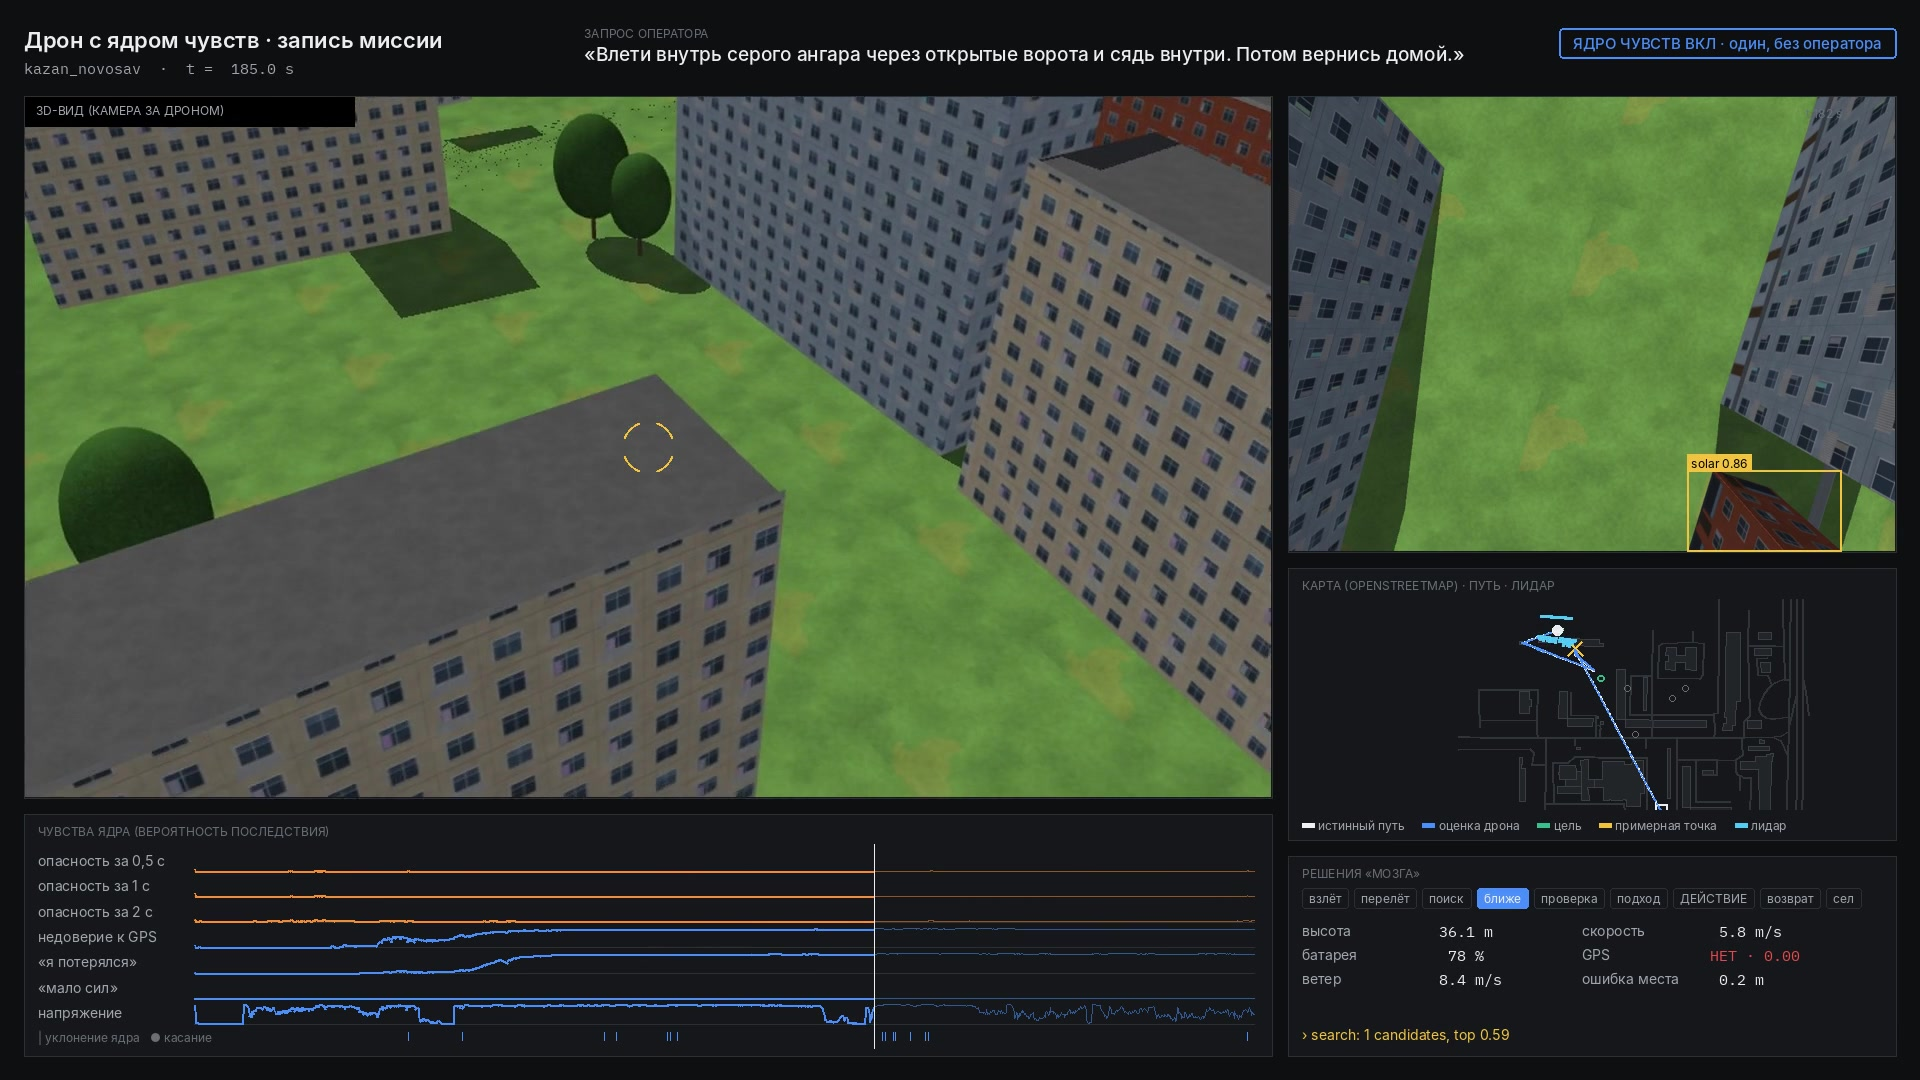
\includegraphics[width=\linewidth]{frame_mission_ru.jpg}
\caption{Кадр миссии G45 (влететь в серый ангар и вернуться домой) в казанском районе проверки, 185\,с полёта. GPS пропал на
36\,с, дрон летит по лидару и карте, и его чувство «я потерялся» выросло. Слева вид сзади и чувства ядра за весь полёт с
моментами, когда оно перехватывало команду мозга. Справа камера дрона с найденными объектами, карта с истинным путём, собственной
оценкой дрона и примерной точкой, а ниже этап и состояние мозга миссии.}
\label{fig:frame}
\end{figure}

\begin{figure}[h]
\centering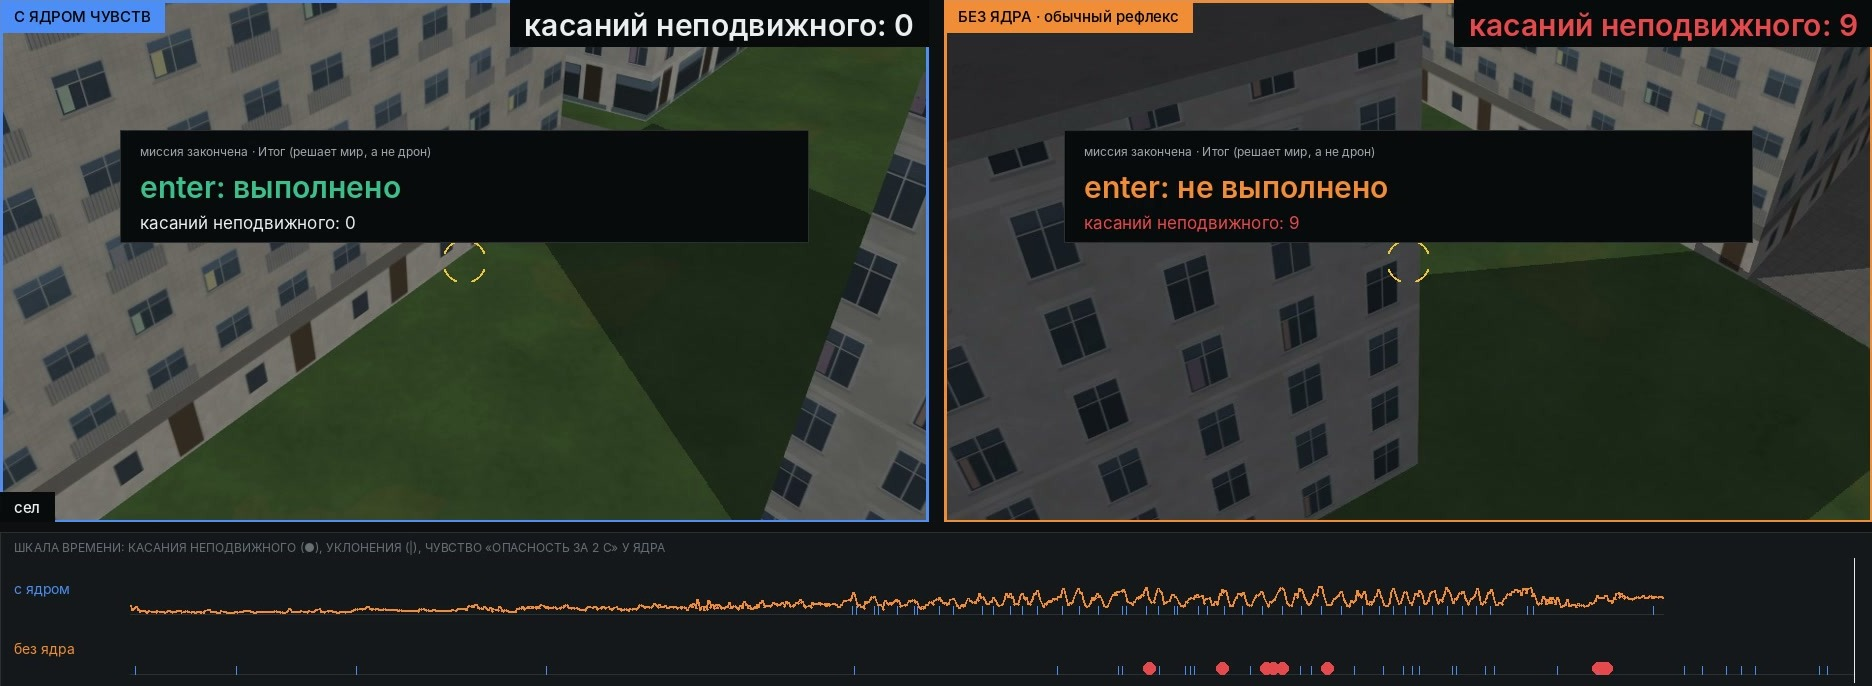
\includegraphics[width=\linewidth]{fig_compare_ru.jpg}
\caption{Кадр видео «рядом» для миссии G206 (влететь в синий ангар, токийский район проверки): одна и та же миссия с ядром чувств
(слева) и с обычным рефлексом вместо него (справа), в конце миссии. С ядром дрон влетел в ангар, ничего не задев; с рефлексом влёт
не удался после 9 касаний неподвижного. Внизу шкала всего полёта: касания неподвижного у каждого дрона (красные точки) и чувство
ядра «опасность за 2\,с». Четыре видео «рядом»~--- это повторы миссий G2 по их
планам на другой модели видеокарты; малые численные различия детектора меняют ход полёта, поэтому повтор в деталях отличается от
записанного полёта G2. На четырёх повторах у ядра 1 касание неподвижного, у рефлекса 16; в одном из них (G112) разницы нет, а в
другом (G45) ядро не выполнило влёт в ангар, который рефлекс сделал ценой 6 касаний.}
\label{fig:compare}
\end{figure}

\begin{figure}[h]
\centering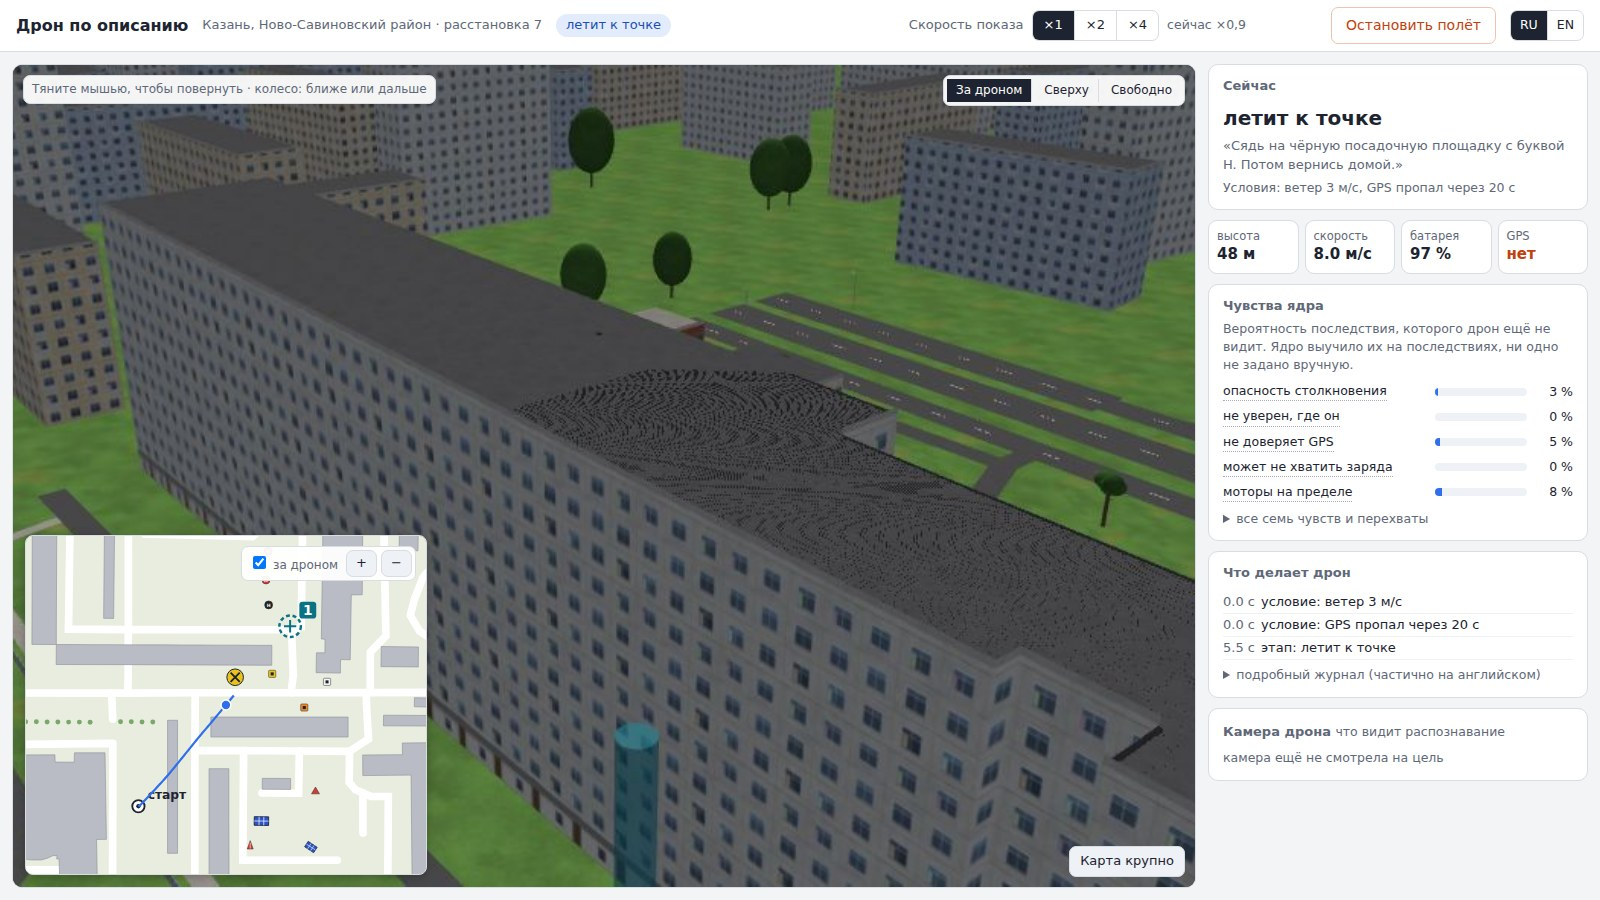
\includegraphics[width=\linewidth]{fig_app_ru.jpg}
\caption{Приложение в полёте. Крупный 3D-вид за дроном рисует сам симулятор; карта в углу показывает примерную точку, истинный путь
и собственную оценку дрона. Справа этап полёта, условия (здесь GPS пропал через 20\,с), высота, скорость, батарея и GPS, пять
чувств ядра и лента событий. До полёта оператор ставит примерную точку, пишет задание, проверяет разбор, показанный простыми
словами, и выбирает условия.}
\label{fig:app}
\end{figure}

